\documentclass[a4paper, oneside]{article}
\usepackage[english, russian]{babel}

\usepackage{fontspec}
\setmainfont[
  Ligatures=TeX,
  Extension=.otf,
  BoldFont=cmunbx,
  ItalicFont=cmunti,
  BoldItalicFont=cmunbi,
]{cmunrm}
\usepackage{unicode-math}

\usepackage[bookmarks=false]{hyperref}
\hypersetup{pdfstartview={FitH},
            pdfauthor={Павел Соболев}}

\usepackage[lmargin=23mm]{geometry}

\usepackage[table]{xcolor}
\usepackage{booktabs}
\usepackage{caption}

\usepackage{graphicx}
\graphicspath{ {./figures/} }

\usepackage{sectsty}
\sectionfont{\centering}
\subsubsectionfont{\centering \vspace{-0.5em}\normalfont\itshape}

\newcommand{\npar}{\par\vspace{\baselineskip}}
\newcommand{\su}{\vspace{-0.5em}}
\newcommand{\sd}{\vspace{0.5em}}

\setlength{\parindent}{0pt}

\hypersetup{pdftitle={Астрофизическая практика: отчет по пятой работе}}

\begin{document}

\section*{Работа №5: Построение кривой блеска и \\ определение параметров поляризации}
\subsubsection*{Выполнил: Павел Соболев}

\vspace{3em}

\subsection*{Задачи}

\begin{itemize}
  \setlength\itemsep{-0.1em}
  \item Используя данные выбранного объекта, измерить видимые R, I звездные величины и параметры поляризации;
  \item Построить кривые блеска для каждого из фильтров в соотношении со стандартом;
  \item Построить график зависимости степени поляризации от даты;
  \item Проанализировать, наблюдается ли корреляция между значениями кривой блеска и степенями поляризации.
\end{itemize}

\subsection*{Ход выполнения и результаты}

В ходе обработки данных Лацертиды (BL Lacertae) были получены следующие данные:

\begin{table}[h]
  \centering
  \caption{Видимые звездные величины объекта в фильтрах R и I (часть 1)}
  \begin{tabular}{ccccccc}
    \toprule
    JD (R) &
    R &
    $\sigma$R &
    JD (I) &
    I &
    $\sigma$I &
    R\,-I \\
    \midrule
    56536.3558 & 13.7460 & 0.0090 & 56536.3585 & 12.7920 & 0.0070 & 0.9540 \\
    \arrayrulecolor{black!40}
    \midrule
    56540.4226 & 14.0420 & 0.0070 & 56540.4283 & 13.1880 & 0.0040 & 0.8540 \\
    \midrule
    56541.3018 & 13.9430 & 0.0050 & 56541.3046 & 13.1150 & 0.0040 & 0.8280 \\
    \midrule
    56542.5013 & 13.9610 & 0.0050 & 56542.5060 & 13.0970 & 0.0040 & 0.8640 \\
    \midrule
    56543.3541 & 13.9590 & 0.0050 & 56543.3568 & 13.0980 & 0.0030 & 0.8610 \\
    \midrule
    56545.3668 & 14.0490 & 0.0060 & 56545.3697 & 13.0830 & 0.0040 & 0.9660 \\
    \midrule
    56546.3152 & 13.7970 & 0.0050 & 56546.3180 & 12.9690 & 0.0030 & 0.8280 \\
    \midrule
    56547.3304 & 13.6750 & 0.0040 & 56547.3354 & 12.7810 & 0.0030 & 0.8940 \\
    \midrule
    56549.2789 & 13.5480 & 0.0040 & 56549.2818 & 12.7300 & 0.0030 & 0.8180 \\
    \midrule
    56550.3737 & 13.5830 & 0.0040 & 56550.3764 & 12.7200 & 0.0030 & 0.8630 \\
    \midrule
    56552.3870 & 13.5410 & 0.0040 & 56552.3919 & 12.6760 & 0.0030 & 0.8650 \\
    \midrule
    56569.4054 & 13.5210 & 0.0040 & 56569.4087 & 12.7030 & 0.0030 & 0.8180 \\
    \midrule
    56577.3632 & 13.2990 & 0.0060 & 56577.3684 & 12.4990 & 0.0040 & 0.8000 \\
    \midrule
    56578.1791 & 13.1860 & 0.0130 & 56578.1912 & 12.4130 & 0.0030 & 0.7730 \\
    \midrule
    56580.3644 & 13.3850 & 0.0030 & 56580.3671 & 12.5610 & 0.0020 & 0.8240 \\
    \midrule
    56585.3955 & 13.1770 & 0.0030 & 56585.3982 & 12.3470 & 0.0020 & 0.8300 \\
    \midrule
    56586.2477 & 13.1650 & 0.0030 & 56586.2517 & 12.3550 & 0.0020 & 0.8100 \\
    \midrule
    56588.2350 & 13.3790 & 0.0050 & 56588.2377 & 12.5410 & 0.0040 & 0.8380 \\
    \arrayrulecolor{black}
    \bottomrule
  \end{tabular}
\end{table}

\newpage

\begin{table}[h]
  \centering
  \caption{Видимые звездные величины объекта в фильтрах R и I (часть 2)}
  \begin{tabular}{ccccccc}
    \toprule
    JD (R) &
    R &
    $\sigma$R &
    JD (I) &
    I &
    $\sigma$I &
    R\,-I \\
    \midrule
    56591.3998 & 13.2820 & 0.0030 & 56591.4194 & 12.4730 & 0.0020 & 0.8090 \\
    \arrayrulecolor{black!40}
    \midrule
    56597.1685 & 12.8060 & 0.0030 & 56597.1715 & 12.0380 & 0.0020 & 0.7680 \\
    \midrule
    56602.3555 & 13.1470 & 0.0020 & 56602.3584 & 12.3430 & 0.0020 & 0.8040 \\
    \midrule
    56605.2586 & 12.8570 & 0.0020 & 56605.2841 & 12.0460 & 0.0020 & 0.8110 \\
    \midrule
    56608.1664 & 13.2440 & 0.0030 & 56608.1693 & 12.4410 & 0.0020 & 0.8030 \\
    \midrule
    56615.1514 & 13.2540 & 0.0030 & 56615.1723 & 12.4230 & 0.0030 & 0.8310 \\
    \midrule
    56621.2505 & 12.6410 & 0.0020 & 56621.2532 & 11.8660 & 0.0010 & 0.7750 \\
    \midrule
    56623.1098 & 12.7320 & 0.0030 & 56623.1139 & 11.9390 & 0.0020 & 0.7930 \\
    \midrule
    56631.3270 & 13.1630 & 0.0030 & 56631.3299 & 12.3420 & 0.0020 & 0.8210 \\
    \midrule
    56640.1457 & 13.7100 & 0.0050 & 56640.1492 & 12.8670 & 0.0030 & 0.8430 \\
    \midrule
    56641.1475 & 13.3790 & 0.0040 & 56641.1506 & 12.5830 & 0.0030 & 0.7960 \\
    \arrayrulecolor{black}
    \bottomrule
  \end{tabular}
\end{table}

\begin{table}[h]
  \centering
  \caption{Степени и углы поляризации объекта (часть 1)}
  \begin{tabular}{ccccccc}
    \toprule
    JD &
    m &
    P &
    $\sigma$P &
    PA &
    $\sigma$PA &
    FWHM \\
    \midrule
    56536.3634 & 13.6705 & 0.6914 & 1.4793 & 140.6096 & 61.4042 & 2.1475 \\
    \arrayrulecolor{black!40}
    \midrule
    56540.4348 & 13.9200 & 4.8775 & 1.0199 & 169.0117 & 6.0012 & 1.9563 \\
    \midrule
    56541.3129 & 13.8915 & 3.2152 & 1.7247 & 7.1903 & 15.3950 & 1.9462 \\
    \midrule
    56542.5114 & 13.8355 & 5.4152 & 1.5334 & 158.2911 & 8.1268 & 1.9813 \\
    \midrule
    56543.3620 & 13.8675 & 10.1796 & 0.7187 & 150.5006 & 2.0264 & 2.1850 \\
    \midrule
    56545.3768 & 13.8780 & 15.3213 & 2.8278 & 162.6254 & 5.2971 & 1.9325 \\
    \midrule
    56546.3229 & 13.7575 & 12.4428 & 2.3806 & 150.0168 & 5.4909 & 2.0025 \\
    \midrule
    56547.3473 & 13.6090 & 14.6659 & 2.3789 & 161.5024 & 4.6553 & 1.9588 \\
    \midrule
    56549.2873 & 13.4665 & 11.2744 & 1.5462 & 141.3837 & 3.9360 & 2.0075 \\
    \arrayrulecolor{black}
    \bottomrule
  \end{tabular}
\end{table}

\newpage

\begin{table}[h]
  \centering
  \caption{Степени и углы поляризации объекта (часть 2)}
  \begin{tabular}{ccccccc}
    \toprule
    JD &
    m &
    P &
    $\sigma$P &
    PA &
    $\sigma$PA &
    FWHM \\
    \midrule
    56550.3813 & 13.4765 & 9.9617 & 1.2404 & 156.8403 & 3.5736 & 2.1537 \\
    \arrayrulecolor{black!40}
    \midrule
    56552.3971 & 13.4075 & 12.4410 & 0.9988 & 165.5077 & 2.3041 & 2.0625 \\
    \midrule
    56569.4146 & 13.4940 & 11.4891 & 1.0966 & 167.2973 & 2.7392 & 1.9925 \\
    \midrule
    56577.3847 & 13.2490 & 12.1699 & 1.4052 & 173.9112 & 3.3138 & 2.0250 \\
    \midrule
    56578.1851 & 13.1785 & 10.2769 & 0.7384 & 178.2259 & 2.0621 & 2.0525 \\
    \midrule
    56580.3721 & 13.3010 & 2.9258 & 0.9708 & 14.3813 & 9.5232 & 2.2112 \\
    \midrule
    56585.4175 & 13.1090 & 0.4402 & 1.1097 & 144.0068 & 72.3504 & 2.1625 \\
    \midrule
    56586.2331 & 13.0810 & 1.3070 & 0.6599 & 118.1502 & 14.4896 & 2.2775 \\
    \midrule
    56588.2425 & 13.2775 & 1.0461 & 0.7691 & 136.1884 & 21.1001 & 2.5575 \\
    \midrule
    56591.4052 & 13.2495 & 10.0611 & 1.0264 & 9.7501 & 2.9278 & 1.9875 \\
    \midrule
    56597.1839 & 12.7745 & 7.6083 & 0.3221 & 182.0373 & 1.2150 & 2.3400 \\
    \midrule
    56602.3644 & 13.0600 & 5.8633 & 0.4352 & 31.6716 & 2.1304 & 2.3800 \\
    \midrule
    56605.2773 & 12.7875 & 8.0028 & 0.3421 & 67.6820 & 1.2270 & 2.2675 \\
    \midrule
    56608.1600 & 13.1820 & 12.1093 & 0.5322 & 56.5424 & 1.2614 & 2.2050 \\
    \midrule
    56615.1587 & 13.1835 & 12.6558 & 0.6592 & 12.7137 & 1.4949 & 2.6412 \\
    \midrule
    56621.2582 & 12.5450 & 8.6208 & 0.2372 & 29.1651 & 0.7898 & 2.0250 \\
    \midrule
    56623.1202 & 12.6690 & 5.9439 & 0.7510 & 173.9255 & 3.6261 & 2.9037 \\
    \midrule
    56631.3110 & 13.0800 & 20.3393 & 1.2419 & 177.1344 & 1.7524 & 2.0538 \\
    \midrule
    56640.1541 & 13.6340 & 3.3824 & 0.7550 & 153.7711 & 6.4061 & 2.3363 \\
    \midrule
    56641.1556 & 13.3140 & 2.3131 & 0.8012 & 156.2109 & 9.9406 & 2.1563 \\
    \arrayrulecolor{black}
    \bottomrule
  \end{tabular}
\end{table}

\newpage

\begin{table}[h]
  \centering
  \caption{Степени и углы поляризации первого стандарта (часть 1)}
  \begin{tabular}{ccccccc}
    \toprule
    JD &
    m &
    P &
    $\sigma$P &
    PA &
    $\sigma$PA &
    FWHM \\
    \midrule
    56536.3634 & 11.9985 & 2.3024 & 0.1443 & 38.2082 & 1.7982 & 2.1725 \\
    \arrayrulecolor{black!40}
    \midrule
    56540.4348 & 11.9925 & 0.5807 & 0.1701 & 151.2029 & 8.4074 & 1.99 \\
    \midrule
    56541.3129 & 12.0025 & 2.854 & 0.0948 & 92.7309 & 0.953 & 2.0075 \\
    \midrule
    56542.5114 & 11.9845 & 2.4893 & 0.1032 & 160.1171 & 1.1903 & 1.9675 \\
    \midrule
    56543.362 & 12.003 & 0.8625 & 0.0983 & 166.1785 & 3.2708 & 2.2025 \\
    \midrule
    56545.3768 & 11.9995 & 4.8046 & 0.1019 & 27.837 & 0.6085 & 1.9675 \\
    \midrule
    56546.3229 & 11.9865 & 4.0206 & 0.1082 & 179.3286 & 0.7724 & 1.9875 \\
    \midrule
    56547.3473 & 11.996 & 4.0469 & 0.1047 & 160.3457 & 0.7428 & 1.99 \\
    \midrule
    56549.2873 & 11.9795 & 2.5923 & 0.1018 & 95.5333 & 1.1273 & 1.97 \\
    \midrule
    56550.3813 & 11.9965 & 2.0058 & 0.1184 & 126.3713 & 1.6948 & 2.175 \\
    \midrule
    56552.3971 & 12.004 & 1.5477 & 0.1259 & 98.2877 & 2.334 & 2.075 \\
    \midrule
    56569.4146 & 11.9925 & 1.6999 & 0.128 & 93.3077 & 2.1612 & 2.005 \\
    \midrule
    56577.3847 & 11.995 & 1.4607 & 0.356 & 194.6832 & 6.994 & 2.005 \\
    \midrule
    56578.1851 & 11.9775 & 0.6991 & 0.2067 & 164.2015 & 8.4839 & 2.0725 \\
    \midrule
    56580.3721 & 12.0085 & 1.5602 & 0.1138 & 158.1154 & 2.0942 & 2.2325 \\
    \midrule
    56585.4175 & 12.004 & 1.771 & 0.159 & 130.9586 & 2.5771 & 2.19 \\
    \midrule
    56586.2331 & 12.007 & 1.0254 & 0.1124 & 2.7454 & 3.1475 & 2.325 \\
    \midrule
    56588.2425 & 11.9955 & 1.0479 & 0.1498 & 17.1494 & 4.103 & 2.555 \\
    \midrule
    56591.4052 & 11.9825 & 1.6564 & 0.1201 & 29.3027 & 2.081 & 1.96 \\
    \midrule
    56597.1839 & 11.999 & 0.451 & 0.0962 & 100.7342 & 6.1223 & 2.35 \\
    \midrule
    56602.3644 & 11.9985 & 0.6034 & 0.1025 & 171.4364 & 4.8771 & 2.39 \\
    \arrayrulecolor{black}
    \bottomrule
  \end{tabular}
\end{table}

\newpage

\begin{table}[h]
  \centering
  \caption{Степени и углы поляризации первого стандарта (часть 2)}
  \begin{tabular}{ccccccc}
    \toprule
    JD &
    m &
    P &
    $\sigma$P &
    PA &
    $\sigma$PA &
    FWHM \\
    \midrule
    56605.2773 & 11.9975 & 0.4469 & 0.1119 & 0.0382 & 7.1888 & 2.265 \\
    \arrayrulecolor{black!40}
    \midrule
    56608.16 & 12.0125 & 0.7509 & 0.109 & 10.0366 & 4.1652 & 2.215 \\
    \midrule
    56615.1587 & 12.014 & 0.8929 & 0.1421 & 178.9649 & 4.5686 & 2.6525 \\
    \midrule
    56621.2582 & 11.9825 & 0.22 & 0.1223 & 132.5542 & 15.9533 & 1.96 \\
    \midrule
    56623.1202 & 11.996 & 1.2349 & 0.1296 & 177.3136 & 3.0129 & 2.925 \\
    \midrule
    56631.311 & 12.0015 & 2.1033 & 0.0992 & 88.0951 & 1.353 & 2.0525 \\
    \midrule
    56640.1541 & 12.002 & 0.9688 & 0.1167 & 13.7974 & 3.4563 & 2.3375 \\
    \midrule
    56641.1556 & 11.997 & 1.1075 & 0.1466 & 176.0218 & 3.8004 & 2.1675 \\
    \arrayrulecolor{black}
    \bottomrule
  \end{tabular}
\end{table}

Из этих данных были отброшены несколько точек объекта, имеющих высокие ошибки тех или иных параметров: 1, 3, 15--18. На основе оставшихся данных были получены следующие графики:

\begin{figure}[h]
  \centering
  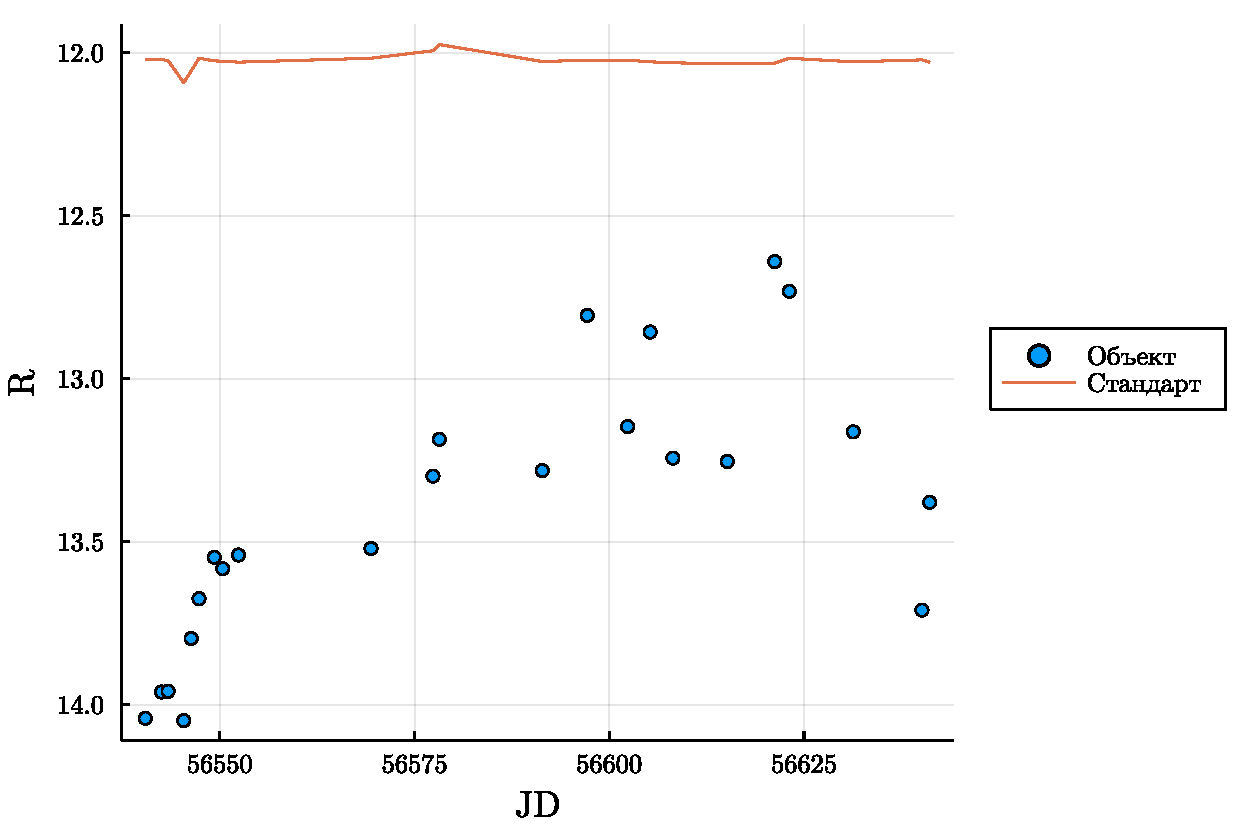
\includegraphics[scale=0.5]{R}
  \caption{Кривая блеска в фильтре R}
\end{figure}

\newpage

\begin{figure}[h!]
  \centering
  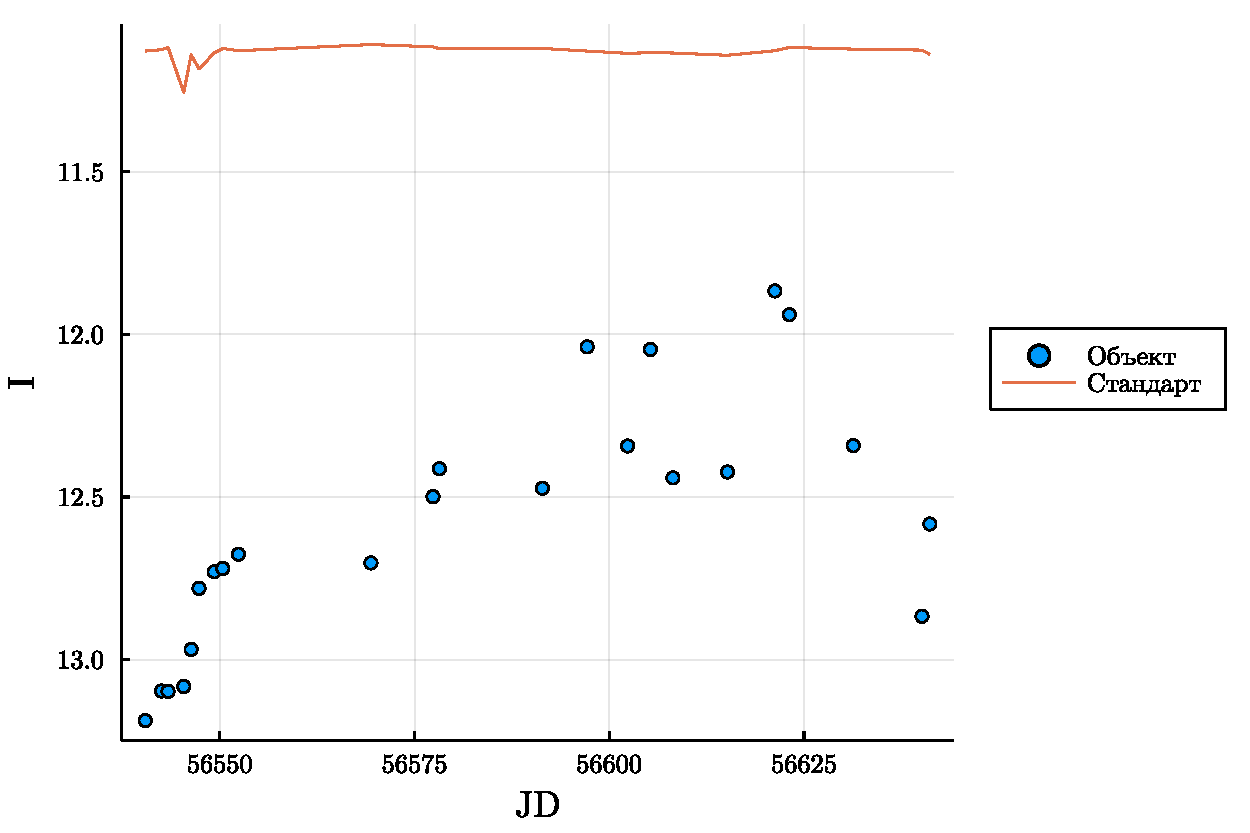
\includegraphics[scale=0.5]{I}
  \caption{Кривая блеска в фильтре I}
\end{figure}

\begin{figure}[h!]
  \centering
  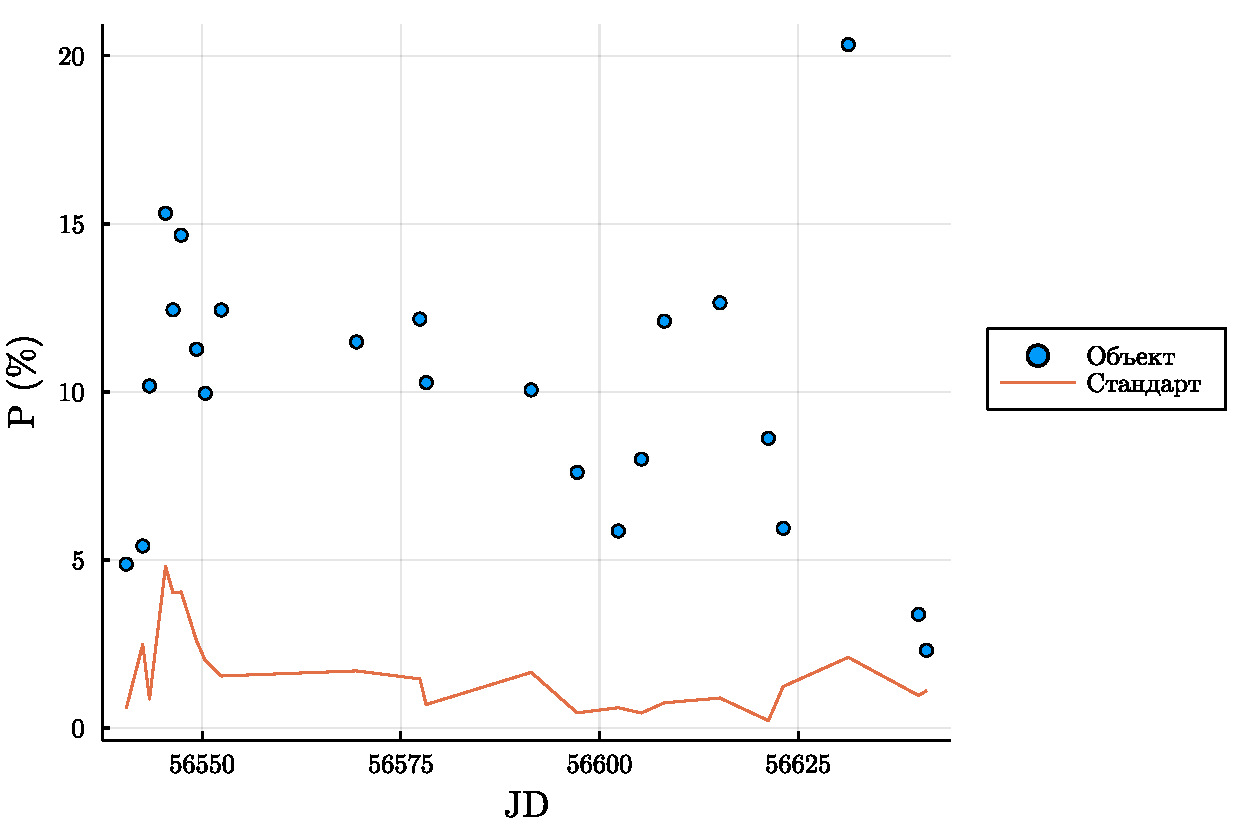
\includegraphics[scale=0.5]{P}
  \caption{Зависимость степени поляризации от даты}
\end{figure}

\newpage

\begin{figure}[h]
  \centering
  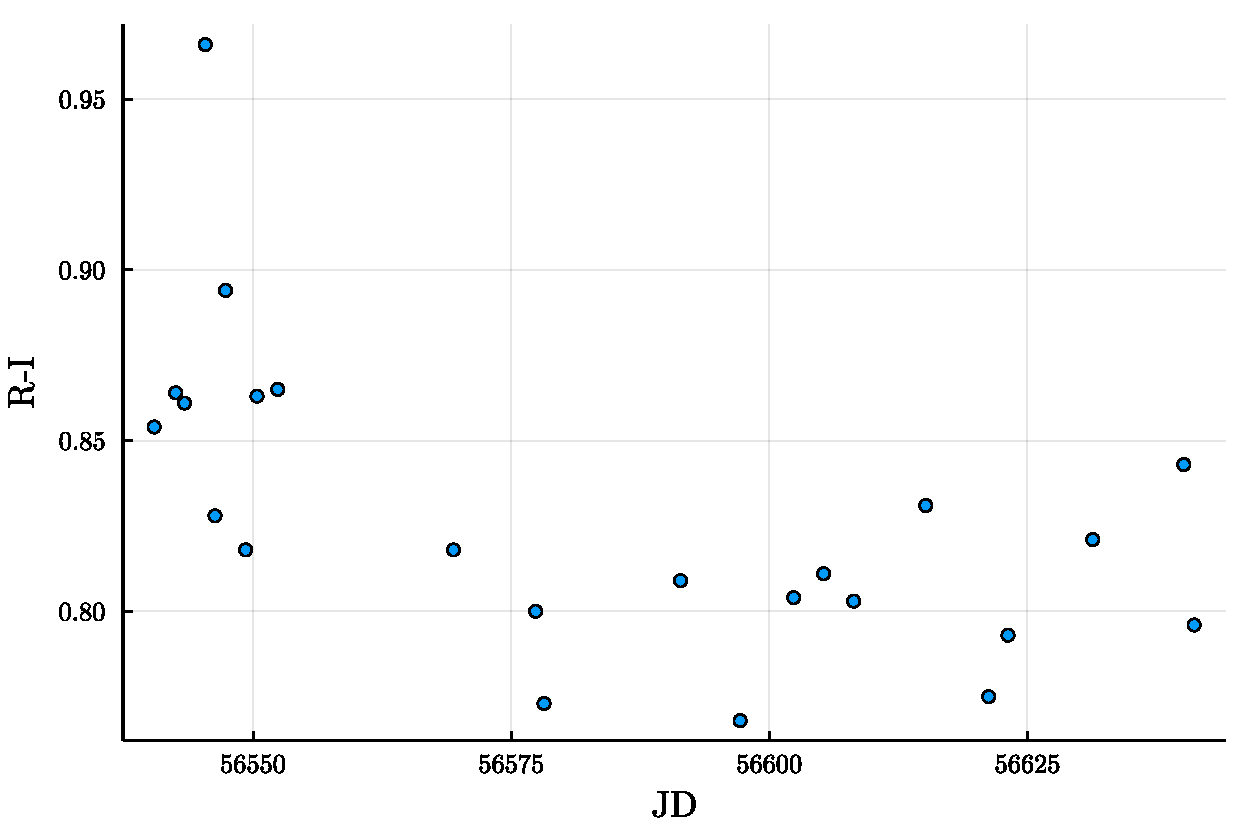
\includegraphics[scale=0.5]{R-I}
  \caption{Зависимость показателя цвета от даты}
\end{figure}

Между значениями звездных величин и поляризацией наблюдаются следующие корреляции:

\begin{itemize}
  \setlength\itemsep{-0.1em}
  \item Участки постоянства значений на промежутке от первого отсчета даты до дня 56575 (с учетом компенсации ошибки в данных, выражающейся в резком повышении звездной величины стандарта);
  \item Медленное убывание значения звездной величины на промежутке от дня 56575 до дня 56590; убывание степени поляризации на том же промежутке;
  \item Локальные минимумы значения звездной величины на днях 56600, 56620; локальные минимумы у степени поляризации там же;
  \item Локальные максимумы значения звездной величины на днях 56617, 56630; локальные максимумы у степени поляризации там же.
\end{itemize}

\end{document}